\documentclass{article}
\usepackage[utf8]{inputenc}
\usepackage[left=1cm,right=0.5cm,bottom=0.5cm,top=0.5cm]{geometry}
\usepackage{setspace}
\usepackage{graphicx}
\usepackage{amsmath}
\usepackage{graphbox}
\usepackage{enumitem}
\setstretch{0.8}
\setlist{nosep}

% 2 sides of paper max
\begin{document}
\begin{center}
    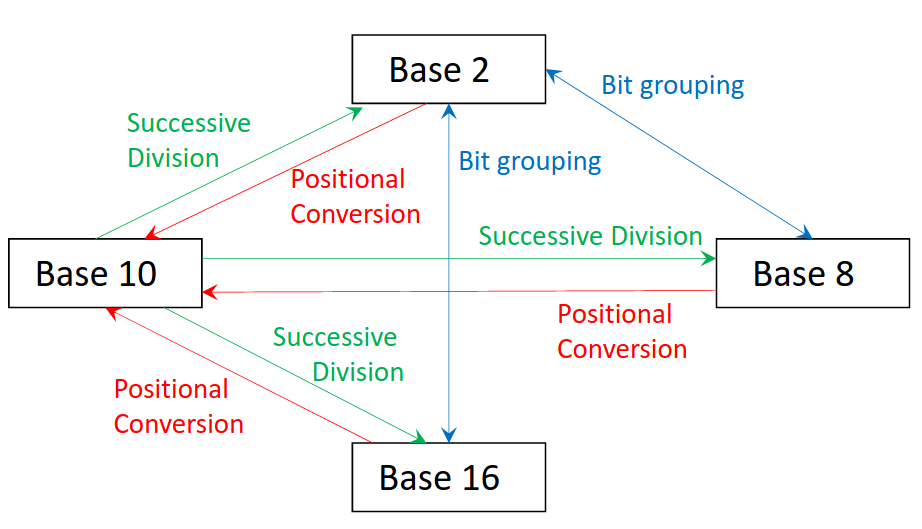
\includegraphics[align=c, width=10cm]{conversions.png}
    \hspace{2cm}
    \begin{tabular}{|c|c|c|c|}
        \hline
        Binary & Octal & Decimal & Hex \\
        \hline
        % Generated with Python lol
        0000 & 00 & 00 & 0 \\
        0001 & 01 & 01 & 1 \\
        0010 & 02 & 02 & 2 \\
        0011 & 03 & 03 & 3 \\
        0100 & 04 & 04 & 4 \\
        0101 & 05 & 05 & 5 \\
        0110 & 06 & 06 & 6 \\
        0111 & 07 & 07 & 7 \\
        1000 & 10 & 08 & 8 \\
        1001 & 11 & 09 & 9 \\
        1010 & 12 & 10 & A \\
        1011 & 13 & 11 & B \\
        1100 & 14 & 12 & C \\
        1101 & 15 & 13 & D \\
        1110 & 16 & 14 & E \\
        1111 & 17 & 15 & F \\
        \hline
    \end{tabular}
\end{center}
\textbf{Base conversion}
\begin{itemize}
    \item Decimal to base $n$:
    \begin{itemize}
        \item Successive division: divide the target number by $n$ and collect the remainders, until the number reaches 0. The converted number should be the remainders, from last to first.
        \item Ex. $(8)_{10} \rightarrow 4 r 0, 2 r 0, 1 r 0, 0 r 1 \rightarrow (1000)_2$
    \end{itemize}
    \item Base $n$ to decimal:
    \begin{itemize}
        \item Positional conversion: multiply each number with the corresponding power of $n.$
        \item Ex. $(1000)_2 = 0 \cdot 2^0 + 0 \cdot 2^1 + 0 \cdot 2^2 + 1\cdot 2^3 = 2^3 = 8$
    \end{itemize}
    \item Binary to/from hex/octal:
    \begin{itemize}
        \item Bit grouping: put bits into groups of 3 (octal) or 4 (hex) and convert using a table.
        \item Ex. $(10111100)_2 = (1011 1100)_2 = (BC)_{16}$
    \end{itemize}
    \item Hex to/from octal:
    \begin{itemize}
        \item Convert to binary and use binary to/from hex/octal.
        \item Ex. $(AF)_{16} = (1010 1111)_2 = (010 101 111)_2 = (257)_8$
    \end{itemize}
\end{itemize}
\textbf{Representing negatives}
\begin{itemize}
    \item Sign magnitude
    \begin{itemize}
        \item Convert the number's absolute value to binary, then stick a 1 in front of it to represent that it's negative
        \item Ex. -8 in 5-bit sign magnitude: $(8)_{10} = (1000)_2 \rightarrow -8 = 11000$
        \item Max value in $n$ bits: $2^{n - 1} - 1$
        \item Min value in $n$ bits: $-2^{n - 1} + 1$
    \end{itemize}
    \item One's complement
    \begin{itemize}
        \item Convert the number's absolute value to binary, then complement all the bits.
        \item Ex. -8 in 5-bit one's complement: $(8)_{10} = (1000)_2 \rightarrow -8 =   \sim 01000 = 10111$
        \item Max value in $n$ bits: $2^{n - 1} - 1$
        \item Min value in $n$ bits: $-2^{n - 1} + 1$
    \end{itemize}
    \item Two's complement
    \begin{itemize}
        \item Convert the number's absolute value to binary, then complement all the bits and add one.
        \item Ex. -8 in 5-bit two's complement: $(8)_{10} = (1000)_2 \rightarrow -8 = (\sim 01000 + 1) = (10111 + 1) = 11000$
        \item Max value in $n$ bits: $2^{n - 1} - 1$
        \item Min value in $n$ bits: $-2^{n - 1}$
        \item Adding and subtracting use the same circuit
        \item Overflow can only occur with 2 positive or negative values. If both values are positive and the output is negative, overflow happened and vice versa.
    \end{itemize}
\end{itemize}
\textbf{Binary coded decimal}
\begin{itemize}
    \item Each decimal digit is represented by 4 bits
    \item Certain range for each digit (A - F or 1010 - 1111) is invalid
    \item To add, we have to skip this range; if the sum of two digits is above 1001 we must add 6 (0110) and propagate the carry to the next set of digits
    \item Ex. 2 + 9 =
    \begin{equation*}
        \begin{array}{cccccc}
            % WORKAROUND: Pandoc has parse errors without these phantom markers
            \phantom{ }  & 0 & 0 & 1 & 0 & \\
            + & 1 & 0 & 0 & 1 & \\
            \hline
            \phantom{ }  & 1 & 0 & 1 & 1 & \\
            + & 0 & 1 & 1 & 0 & \\
            \hline
            \phantom{ }  & 0 & 0 & 0 & 1 & c 1\\
        \end{array}
        = 0001 0001 = (11)_{10}
    \end{equation*}
\end{itemize}
\textbf{Boolean algebra}
\begin{itemize}
    \item Simplification theorems
    \begin{itemize}
        \item $(X \cdot Y) + (X \cdot \overline{Y}) = X$
        \item $(X + Y) \cdot (X + \overline{Y}) = X$
        \item $X + (X \cdot Y) = X$
        \item $X \cdot (X + Y) = X$
        \item $(X + \overline{Y}) \cdot Y = X \cdot Y$
        \item $(X \cdot \overline{Y}) + Y = X + Y$
    \end{itemize}
    \item Demorgan's law: $\overline{(X + Y)} = \overline{X} \cdot \overline{Y}$, $\overline{(X \cdot Y)} = \overline{X} + \overline{Y}$
    \item Consensus theorem
    \begin{itemize}
        \item $X \cdot Y + Y \cdot Z + \overline{X} \cdot Z = X \cdot Y + \overline{X} \cdot Z$
        \item $(X + Y) \cdot (Y + Z) \cdot (\overline{X} + Z) = (X + Y) \cdot (\overline{X} + Z)$
    \end{itemize}
    \item There are $2^{2^n}$ possible functions for $n$ one-bit inputs.
\end{itemize}
\textbf{Two-level logic}
\begin{itemize}
    \item Minterm: an AND of each input together, complemented if its value is 0.
    \item Sum of Products: minterms added together to represent a function. 0 outputs are excluded.
    \item Maxterm: an OR of each input together, complemented if its value is 1.
    \item Product of Sums: maxterms multiplied together to represent a function. 1 outputs are excluded.
\end{itemize}
\textbf{K-maps}
\begin{itemize}
    \item You can ONLY group bits in sizes of $2^n$.
    \item You can ONLY group bits in rectangles / squares.
    \item Maps overflow back around the edges.
    \item SOP form: simply circle the largest groups of 1s and see which variables have to be on or off for the range to work. Each group is a SOP term and multiplied together to form the function..
    \item POS form: circle the largest groups of 0s and see which variables have to be on or off to work. Each group is a POS term (inverted!) and added together to form the function.
\end{itemize}
\textbf{Sequential logic}
\begin{itemize}
    \item lzskdjflsdkfj
\end{itemize}
\end{document}
